
\chapter{Overview of ZMathLang}
\label{ch:design}

Using the methodology of MathLang for mathematics (section \ref{sec:mathlangbackground}),
I have created and implemented a step by step way of translating Z
specifications into theorem provers with additional checks for correctness along
the way. This translation consists of one large framework (executed by a user
interface) with many smaller tools to assist the translation. Not only is the
translation useful for a novice to translate a formal specification into a
theorem prover but it also creates other diagrams and graphs to help with the
analysis of a formal system specification.

\begin{figure}[H]
 \begin{center}
 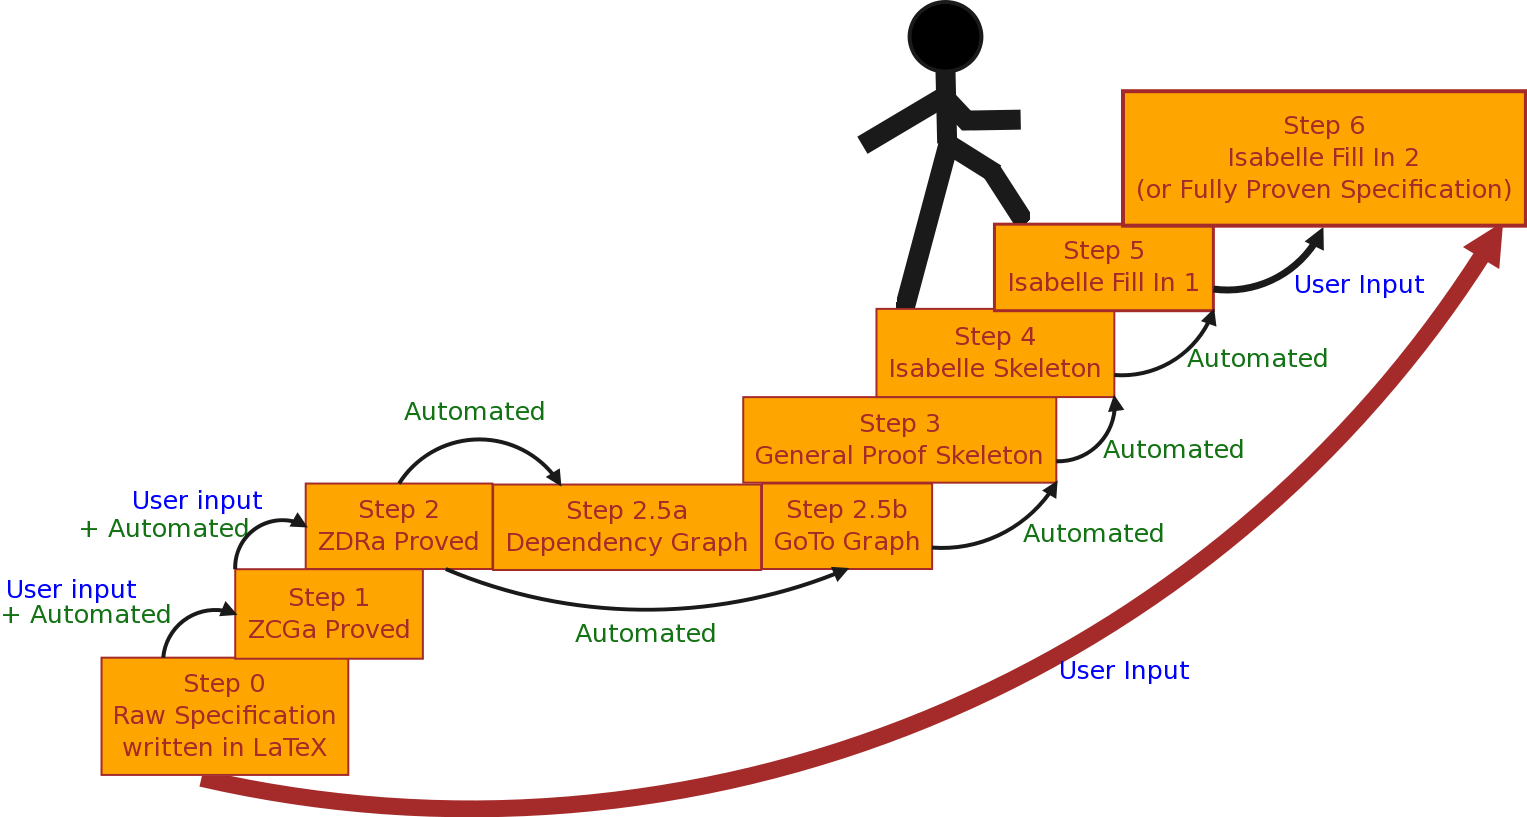
\includegraphics [width=12cm]{Figures/Design/mathlangsteps.png}
 \caption{The steps required to obtain a full proof from a raw specification.}
 \label{fig:steps}
\end{center}
\end{figure} 

The framework is targeted at beginners in theorem proving. The users should have
some idea of formal specifications but have no or little knowledge of the
targeted theorem prover. Figure \ref{fig:steps} shows the outline of the
framework. The higher the user goes up the steps the more rigorous the checks
for correctness. Step 1 and step 2 are interchangeable and can be done in any
order. However they both must be completed before moving up to step 3. Step 6 is
the highest level of rigour and checks for full correctness in a theorem prover.
For this thesis I have chose to translate Z specifications into Isabelle,
however this framework is an outline for any formal specification into any
theorem prover which could done in the future.

The user doesn't need to go all the way to the top to check for correctness, one
advantage of breaking up the translation is that the user gets some level of
rigour and can be satisfied with some level of correctness along the way.
However the main advantage of breaking up the translation is that the level of
expertise needed to check for the correctness of a system specification can be
done by someone who is not a theorem prover expert. This tool could also aid
users in learning theorem proving as it translates their specification and thus
they have examples of the syntax used in their theorem prover for their
specification. 

The arrows in figure \ref{fig:steps} represent the amount of expertise needed
for each step. In the last step, the arrow is slightly thicker as perhaps some
theorem prover knowledge would be needed to complete the proofs. However these
arrows are still small in comparison to the red thick arrow which represents
translating the specification all in one go.

The framework breaks the translation into 6 steps, most of which are partially
or fully automated. These are:

\begin{itemize}
\item Step 0: Raw LaTeX Z Specification. {\color{set}Start}
\item Step 1: Check for Core Grammatical correctness (ZCGa). {\color{set}User Input + Automated}
\item Step 2: Check for Document Rhetorical correctness (ZDRa). {\color{set}User Input + Automated}
\item Step 3: Generate a General Proof Skeleton (GPSa). {\color{set}Automated}
\item Step 4: Generate an Isabelle Skeleton. {\color{set}Automated}
\item Step 5: Fill in the Isabelle Skeleton. {\color{set}Automated}
\item Step 6: Prove existing lemmas and add more safety properties if needed. {\color{set}User Input}
\end{itemize}

\section{How far does the automation go?}

Figure \ref{fig:timeline} shows a diagram showing how far one can automate a
specification using automated \gls{zmath} and Isabelle tools. \Gls{zmath} is a
tool-set which assists the user in translating and proving a specification (going
from left to right). There are also other automating tools within Isabelle which
also assist the user with proving specifications (going from right to left) in
the diagram.

\begin{figure}[H]
 \begin{center}
 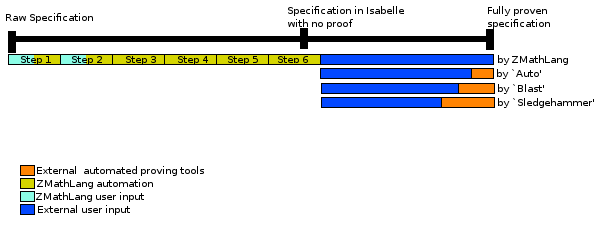
\includegraphics [scale=0.75]{Figures/Design/timeline.png}
 \caption{How far can one automate a specification proof.}
 \label{fig:timeline}
\end{center}
\end{figure} 

In figure \ref{fig:timeline} we show how far the user can get with automation
and how much work is still needed to get the full proof. \Gls{zmath} requires
user input for the first two steps (\gls{zcga} and \gls{zdra}) however the rest
up to step 6 is automated.

The black line shows the path going from a raw specification to a fully proven
specification with a milestone in the middle, which signifies when a
specification has been translated into Isabelle syntax but has no properties or
proof. \Gls{zmath} takes the user a little past this milestone as the tool-set
also generates properties to check the specification for consistency (see
section \ref{sec:proofobl}). These properties are added to the specification
during step 3 and continued throughout the translation. It is important to note
that the \gls{zmath} toolkit adds these properties to the translation but does
not prove them. That is why the rest of the \gls{zmath} path may require
external user input (dark blue) to complete the path. However, the \gls{zmath}
toolkit does assist the user in the translation past the halfway milestone on
the diagram.

We have created the \Gls{zmath} toolkit which assist the user from the
specification to full proof however there is also ongoing research on proving
properties from the theorem prover end. Figure \ref{fig:timeline} shows the
amount of proving techniques each automation holds. We have highlighted that
\gls{zmath} only gets the user so far in their proof however they are free to
use external automated theorem provers in completing their specification proof
if they so wish.

Even external automated theorem provers have their limitations. For example, the
user can use the Isabelle tool `\emph{sledgehammer}' to assist in solving
proofs, but not all can be solved by this technique. The sledgehammer
documentation advises to call `\emph{auto}' or `\emph{safe}' followed by
`\emph{simp\_all}' before invoking sledgehammer. Depending on the complexity of
ones proof, these sometimes may prove the users properties on their own, other
times it may not and the user will still need to invoke sledgehammer to reach
their goal. Sledgehammer itself is a tool that applies \gls{smt} solvers on the
current goal e.g. Vampire\cite{vampire}, SPASS \cite{fmintrol} and E \cite{e}. We
use sledghammer as a collective, to describe all the \gls{smt} solvers it covers
\cite{sledgehammer}.

Other automated methods include:

\begin{itemize}

\item \textbf{simp:} simplifies the current goal using term rewriting.

\item \textbf{arith:} automatically solves linear arithmetic problems.

\item \textbf{clarify:} like `\emph{auto}' but less aggressive.

\item \textbf{clarsimp:} a combination of `\emph{clarify}' and `\emph{simp}'.

\item \textbf{force:} like `\emph{auto}' but only applied to the first goal.

\item \textbf{auto:} applies automated tools to look for a solution.

\item \textbf{blast:} a powerful first-order prover. \cite{isacheat}
\end{itemize}

All these automated tools get increasingly more complex and cover more
properties, e.g \emph{clarsimp} covers more proving techniques then \emph{simp}
and \emph{blast} covers more proving techniques than \emph{auto} etc. With these
tools, one can prove certain properties about their theorem. However, there
still doesn't exist an automated proving tool which covers \textbf{all} proving
techniques. Therefore some user input will be required for more complex proofs.

\section{Overview of ZMathLang step by step}

This section gives an overview of each individual step in the \gls{zmath}
tool-set.

\subsection{Step 0- The raw LaTeX file}

The first step requires the user to write or have a formal specification they
wish to check for correctness. This specification can be fully written in Z or
partially written in Z (thus a specification written in English on it's way to
becoming formalised in Z). The specification should be written in \LaTeX{}
format and can be a mix of natural language and Z syntax. An example of a
specification written in the Z notation can be seen in figure
\ref{fig:zexample}.

\begin{figure}[H]
 \begin{center}
 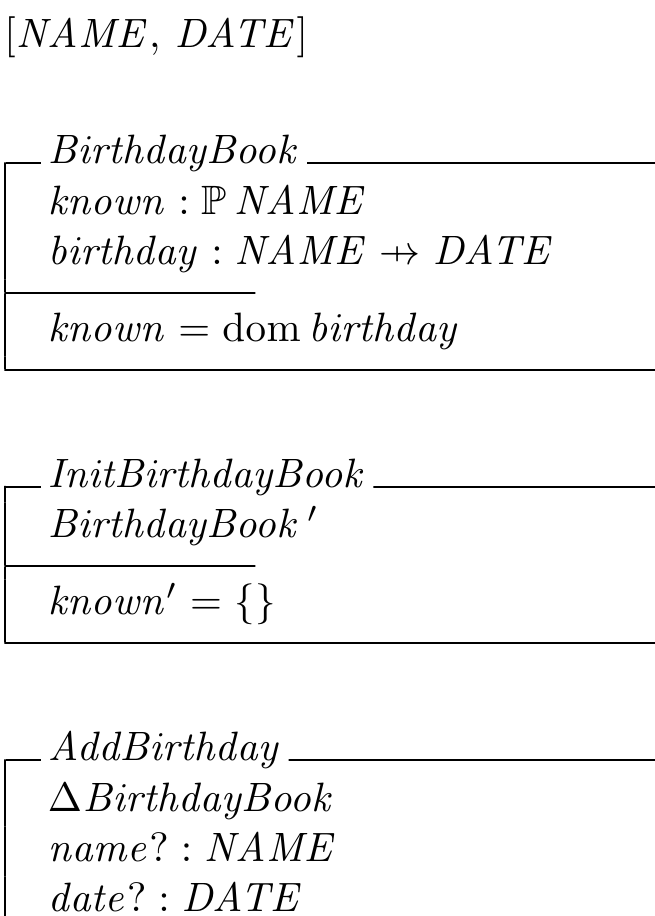
\includegraphics[scale=0.25]{Figures/Design/zspec.png}
 \caption{Example of a partial Z specification.}
 \label{fig:zexample}
\end{center}
\end{figure} 

\subsection{Step 1- The Core Grammatical aspect for Z}

The next step in figure \ref{fig:steps} shows that the specification should be
\gls{zcga} proved. Although this step is interchangeable with step 2 (\gls{zdra})
it is shown as step 2 on the diagram for convenience. In this step the user
annotates their document which they have obtained in step 0 with 7 grammatical
categories and then checks these for correctness. Figure \ref{fig:steps} shows
this step is achieved by user input and automation. The user input of this step
is the annotations and the automation is the \gls{zcga} checker. This
automatically produces a document labeled with the various categories in different
colours and can help identify grammar types to other members in the systems
project team. A \gls{zcga} annotated specification is shown in figure
\ref{fig:zcgaexample}. The \gls{zcga} is further explained in chapter
\ref{ch:zcga}.

\begin{figure}[H]
 \begin{center}
 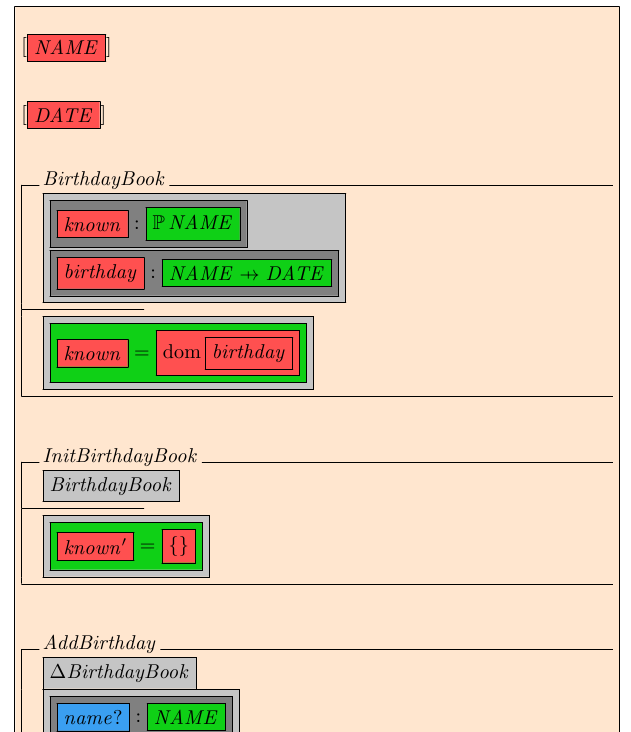
\includegraphics [scale=0.25]{Figures/Design/zcgaexample.png}
 \caption{Example of a ZCGa annotated specification.}
 \label{fig:zcgaexample}
\end{center}
\end{figure} 

\subsection{Step 2- The document Rhetorical aspect for Z}

The \gls{zdra} step, shown as step 2 in figure \ref{fig:steps}, comes before or
after the \gls{zcga} step. Similarly to the \gls{zcga} step, the user annotates
their document from step 0 or step 1 with \gls{zdra} instances and
relationships. This chunks parts of the specification together and allows the
user to describe the relationship between these chunks. The annotation is the
user input part of this step and the automation is the \gls{zdra} checker which
checks if there are any loops in the reasoning and gives warnings if the
specification still needs to be totalised. Once the user has annotated this
document and compiled it, the result shows the specification divided
into chunks and arrows showing the relations between the chunks. An example of a
Z specification annotated in \gls{zdra} is shown in figure
\ref{fig:zdraexample}. The \gls{zdra} is explained further in chapter
\ref{ch:zdra}.

\begin{figure}[H]
 \begin{center}
 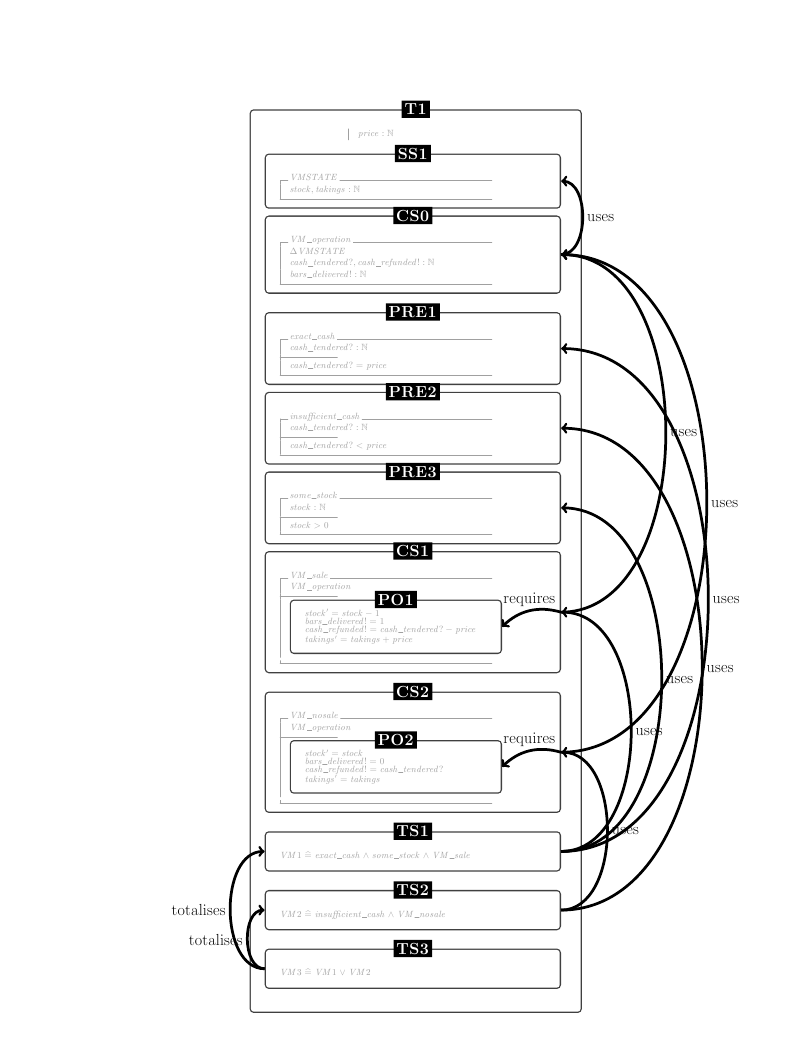
\includegraphics [scale=0.25]{Figures/Design/zdracomp.png}
 \caption{Example of a ZDRa annotated specification.}
 \label{fig:zdraexample}
\end{center}
\end{figure} 

The \gls{zdra} automatically produces a dependency and a goto graph (section
\ref{subsec:zdra_prodcuts}), these are shown as 2.5a and 2.5b respectively in
figure \ref{fig:steps}. The loops in reasoning are checked in both the dependency
graph and goto graph. An example of a goto graph is shown in figure
\ref{fig:gotoexamplee}.

\begin{figure}[H]
 \begin{center}
 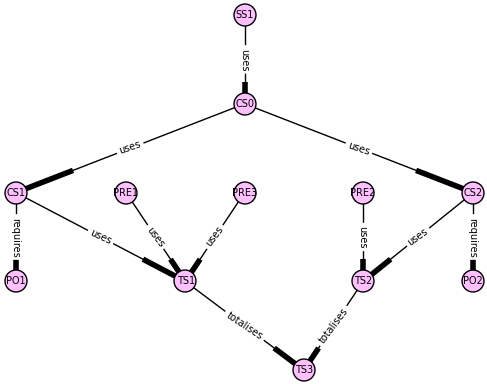
\includegraphics [scale=0.4]{Figures/Design/goto.png}
 \caption{Example of an automatically generated goto graph.}
 \label{fig:gotoexamplee}
\end{center}
\end{figure} 

\subsection{Step 3- The General Proof skeleton}

The following step is an automatically generated \gls{gps}. This document is
automated using the goto graph which is generated from the \gls{zdra} annotated
\LaTeX{} specification. It uses the goto graph to describe in which logical
order to input the specification into any theorem prover. At this stage it also
adds simple proof obligations to check for the consistency of the specification
i.e. the specification is consistent throughout. An example of a general proof
skeleton is shown in figure \ref{fig:proofskelexample}. The \gls{gps} is further
described in section \ref{sec:zdra2gen}.

\begin{figure}[H]
 \begin{center}
 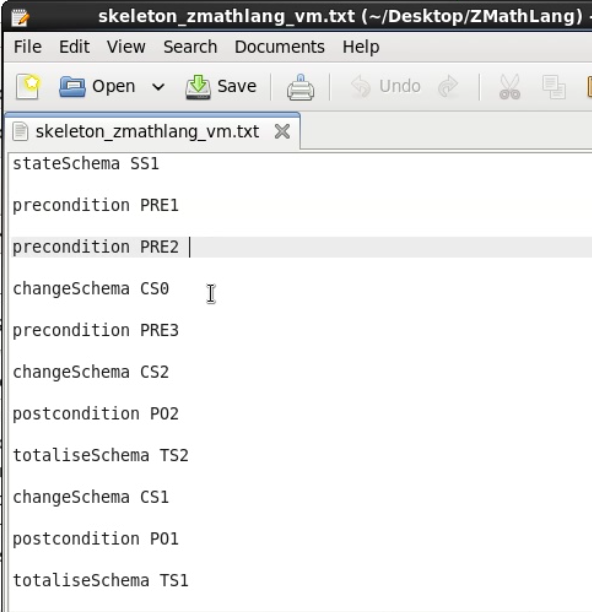
\includegraphics [scale=0.2]{Figures/Design/proofskel.png}
 \caption{Example of a general proof skeleton.}
 \label{fig:proofskelexample}
\end{center}
\end{figure} 

\subsection{Step 4- The Z specification written as an Isabelle Skeleton}

Using the \gls{gps} in step 3, the instances are then translated into an
Isabelle skeleton in step 4. That is, the instances of the specification are
translated into Isabelle syntax using definitions, lemma's, theory's etc to
produce a .thy file. This step is fully automated and thus a user with no
Isabelle experience can still get to this stage. An example of a Z specification
skeleton written in Isabelle is shown in figure \ref{fig:isaskelexample}.
Details of how this translation is conducted is described in chapter
\ref{chap:gpsa2isa} of this thesis.

\begin{figure}[H]
 \begin{center}
 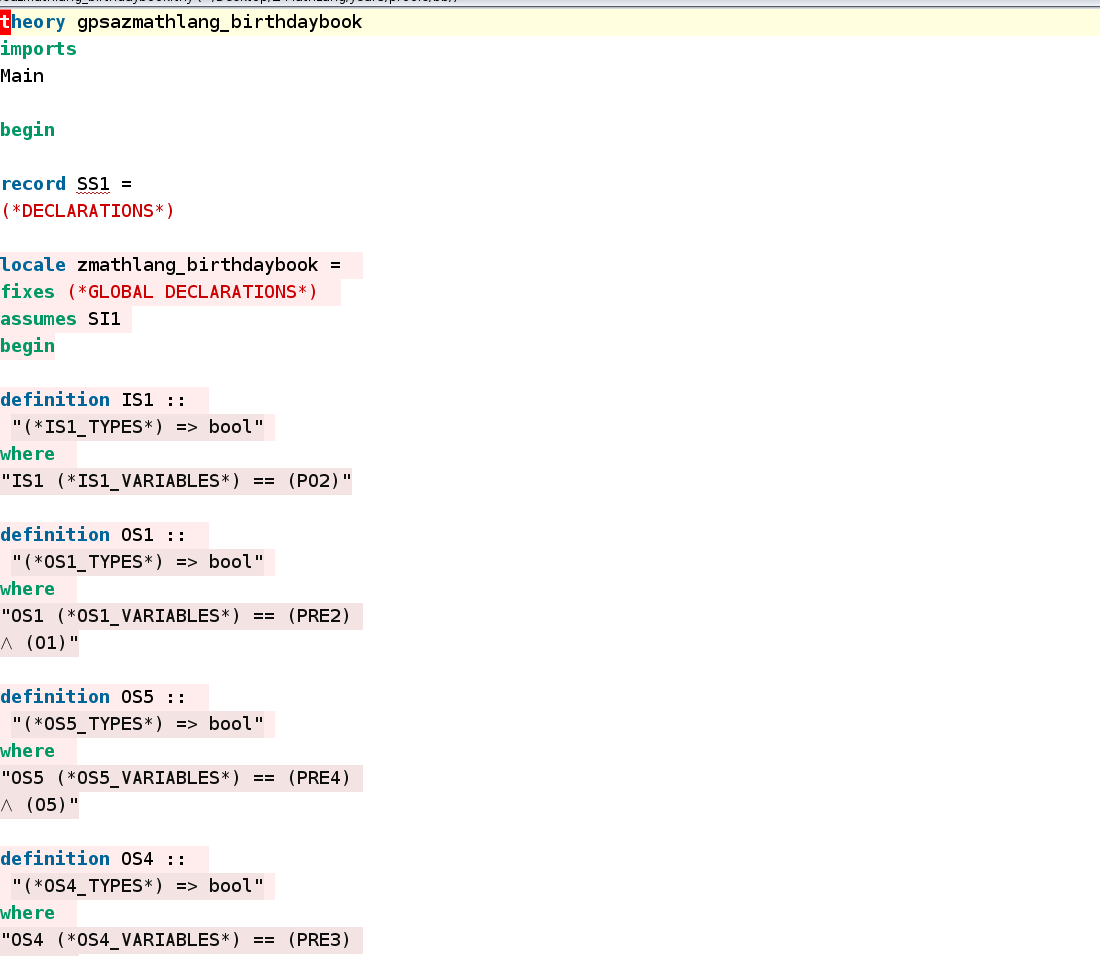
\includegraphics [scale=0.2]{Figures/Design/isaskeleton.png}
 \caption{Example of an Isabelle skeleton.}
 \label{fig:isaskelexample}
\end{center}
\end{figure} 

\subsection{Step 5- The Z specification written as in Isabelle Syntax}

Step 5 is also automated, using the \gls{zcga} annotated document produced in
step 1 and the Isabelle skeleton produced in step 4. This part of the framework
fills in the details from the specification using all the declarations,
expressions, definition etc in Isabelle syntax. Since the translation can also
be done on semi-formal specifications and incomplete formal specification there
may be some information missing in the \gls{zcga} such as an expression or a
definition. Note the lemmas from the proof obligations created in step 3 will
also be filled in, however the actual proofs for these will not and they will be
followed by the command `\texttt{sorry}' to artificially complete the proof. An
example of a filled in isabelle skeleton is shown in figure \ref{fig:fillin1}.

\begin{figure}[H]
 \begin{center}
 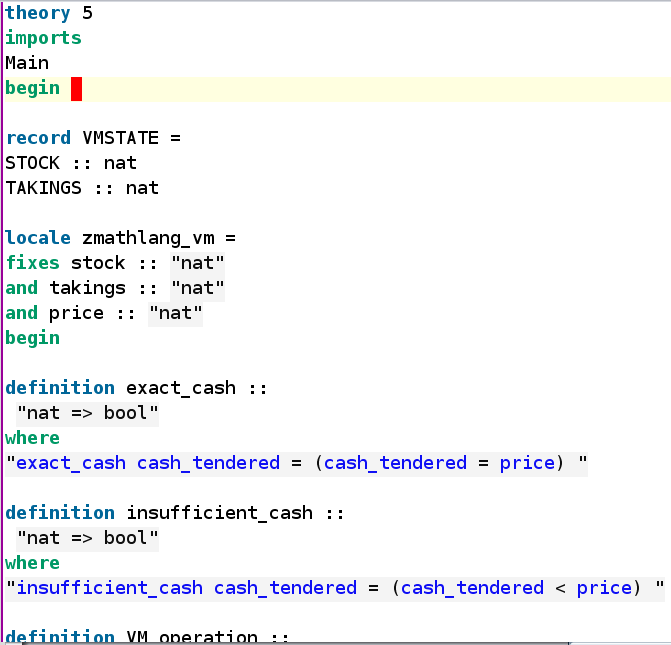
\includegraphics [scale=0.3]{Figures/Design/fillin1.png}
 \caption{Example of an Isabelle skeleton automatically filled in.}
 \label{fig:fillin1}
\end{center}
\end{figure} 

 If there is no \gls{zcga} information to fill in the Isabelle skeleton will not
 change. Further information on the translation is described in section
 \ref{sec:zcga2fillin} of this thesis.

\subsection{Step 6- A fully proven Z specification}

The final step in the \gls{zmath} framework (top of the stairs from figure
\ref{fig:steps}), is to fill in the Isabelle file from step 5. This final step
is represented by a slightly thicker arrow in figure \ref{fig:steps} compared
with the others as the user may need to have some little theorem prover
knowledge to prove properties. Also if there is some missing information such as
missing expressions and definitions the user must fill these out as well in
order to have a fully proven specification. However this may be slightly easier
then writing the specification from scratch as the user would already have
examples of other instances in their Isabelle syntax form. More details on this
last step is described in section \ref{sec:isa2ful} of this thesis.

\section{Procedures and products within ZMathLang}

\begin{figure}[H]
 \begin{center}
 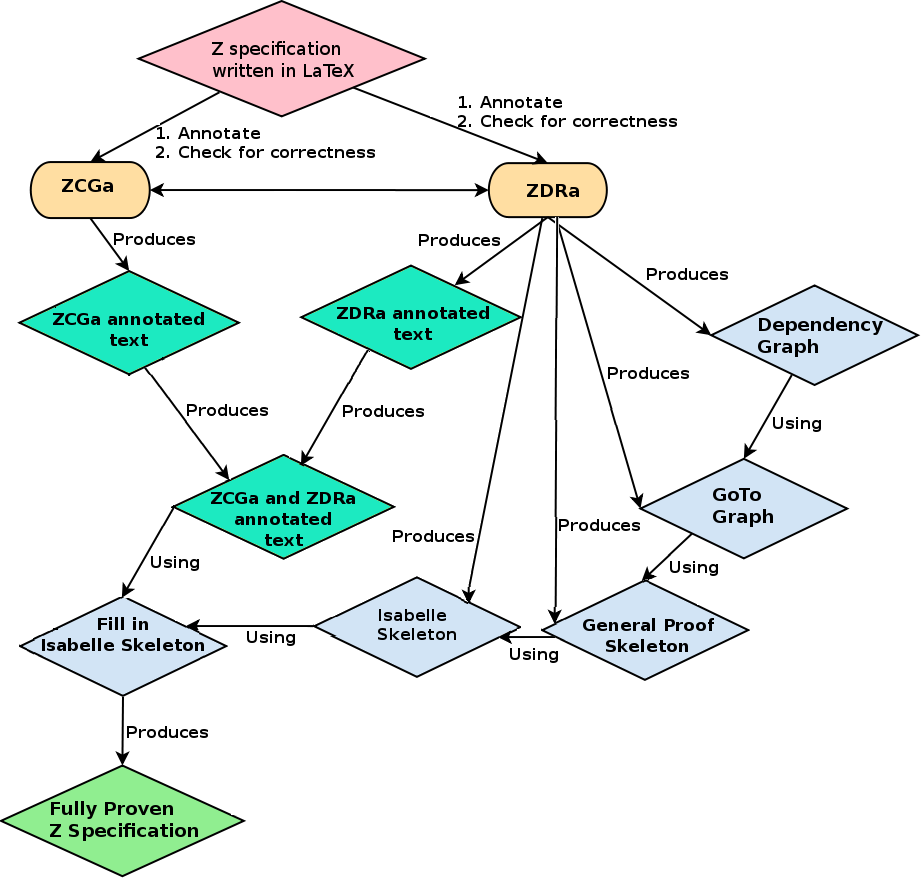
\includegraphics [scale=0.4]{Figures/Design/ZMathLangFlow.png}
 \caption{Flow chart of ZMathLang.}
 \label{fig:zmathflow}
\end{center}
\end{figure} 

Figure \ref{fig:zmathflow} shows a flow chart describing the documents produced
when using the framework and which documents are produced automatically,
semi-automatically and totally by the user. Products which are created by full
automation are diamonds in \colorbox{lightblue}{blue}. Diamonds in
\colorbox{lightgreen}{green} are produced by user input and products shown in
\colorbox{aqua}{aqua} diamonds are partial automated.

The \colorbox{lightpink}{pink} diamond is the starting point for all users. The
\colorbox{lightorange}{orange} ovals describe procedures of the ZCGa and ZDRa.
The ZCGa procedure requires user input and automation to produce a `ZCGa
annotated text'. The ZDRa procedure also requires user input and automation to
produce a `ZDRa annotated text'. Both the \gls{zcga} and \gls{zdra} procedures
done together produce a `\gls{zcga} and \gls{zdra} annotated text'. After
completing the \gls{zdra} procedure a 'dependency graph' is automatically
generated, which can then in turn generate a `GoTo graph' which in turn can
create a general proof skeleton. From the `general proof skeleton' we can then
create an `Isabelle skeleton'  which can be filled in using information from the
`\gls{zcga} and \gls{zdra} annotated text'. Using the `Filled in Isabelle
skeleton' the user needs to fill in the missing information and/or complete the
proofs in order to obtain a `fully proven Z specification'.

\section{The ZMathLang LaTeX Package}

The \gls{zmath} \LaTeX{} package (shown in appendix \ref{app:zmathlatex}) was
implemented to allow the user to label their Z specification document in
\gls{zcga} and \gls{zdra} annotations. Coloured boxes will then appear around
the grammatical categories when the new \gls{zcga} annotated document is
compiled with \texttt{pdflatex}. Instances and labelled arrows showing the
relations are also displayed when annotated with \gls{zdra} and compiled with
\texttt{pdflatex}. 

\subsection{Overview}

The \gls{zmath} style file invokes the following packages:

\begin{itemize}
\item tcolorbox - Used to draw colours around individual grammatical categories
with a black outline for the \gls{zcga}.
\item tikz - Used to identify the instances as nodes so the arrows can join from
one nodes to another.
\item varwidth - Used to chunk each instance as a single entity.
\item zed - Used to draw Z specification schemas, freetypes, axiomatic
definitions in the zed environment.
\item xcolor - Used to define specific colours and gives a wider range of
colours compared to the standard.
\end{itemize}

After invoking the packages we define the colours which are used in the
outputting pdf result. We use the same colours as the original \gls{math}
framework for the grammatical categories which are the same (sets, terms,
expressions, declarations, context and definitions) and choose a different
colour for the weak type `specification' as this hasn't been used in the
original \gls{math} framework.

\begin{figure}[H]

\includegraphics[scale=0.7]{Figures/Design/zmatha.png}
\caption{Part of the syntax to define the colours for \gls{zcga} in the \gls{zmath} \LaTeX{} file. \label{fig:definecolourlatex}}
\end{figure}

The command \verb|\definecolor{*NameOfZCGaType*}{HTML}{*ColourInHtml*}| is used
to define a colour for each grammatical category (shown in figure
\ref{fig:definecolourlatex}). Where \verb|*NameOfZCGaType*| is the name of the
category e.g. definition, term, set etc and \verb|*ColourInHtml*| is the HTML
number for the colour. For example the colour for term in the original
\gls{zmath} is \term{light blue} which in HTML format is \emph{3A9FF1}.
Therefore we define the colour for `\emph{term}' as \emph{3A9FF1}.

\subsection{\LaTeX{} commands to identify ZDRa Instances}

The \gls{zdra} section of the \LaTeX{} file provides three new commands:
\verb|\draschema|, \verb|\draline| and \verb|\dratheory|. The \verb|\dratheory|
annotation is for the entire specification which contains all the instances and
relations. The \verb|\draschema| command is to annotate the instances which are
entire zed schemas, this command should go before any \verb|\begin{schema}| or
\verb|\begin{zed}| command.

\begin{tabular}{|l | l|}
\hline
\verb|\draline{X}{\draschema{Y}{someContext}}| & {\color{set}Incorrect} \\
\hline
\verb|\draschema{Y}{\draline{X}{someContext}}| & {\color{set}Correct} \\
\hline
\end{tabular}

 The \verb|\draline| annotation is to annotate any instance that is a line of
 text which contains plain text or \gls{zcga} annotated text. But does not
 include any \gls{zdra} annotated text. For example in figure
 \ref{fig:zdraincorrectannotations} the \verb|\draline{PRE1}| annotation is
 embedded in the \verb|\draline{CS1}{| which will not compile. Therefore the
 correct way this schema is labelled is shown in figure
 \ref{fig:zdracorrectannotations} where the \verb|\draline{PRE1}| annotation is
 embedded in the \verb|\draschema{CS1}| annotation.

\begin{figure}[H]
\vspace{-0.2in}
\centering
\begin{minipage}{0.45\textwidth}
\centering
\begin{small}
\begin{BVerbatim}
\draline{CS1}{
\begin{schema}{B}
\Delta A
\where
\draline{PRE1}{a<b}
\end{schema}
}
\end{BVerbatim}
\end{small}
\vspace{-0.18in}
\caption{Incorrect annotating of \gls{zdra}.\label{fig:zdraincorrectannotations}}
\vspace{-0.2in}
\end{minipage}\hfill
\begin{minipage}{0.45\textwidth}
\centering
\begin{small}
\begin{BVerbatim}
\draschema{CS1}{
\begin{schema}{B}
\Delta A
\where
\draline{PRE1}{a<b}
\end{schema}
}
\end{BVerbatim}
\end{small}
\vspace{-0.2in}
\caption{Correct annotating of \gls{zdra}.\label{fig:zdracorrectannotations}}
\vspace{-0.2in}
\end{minipage}
\end{figure}

It is important to note this embedding order as by annotating a chunk of
specification using \verb|\draline| keeps everything inside as the \LaTeX{}
`\emph{math mode}'. Since the annotation \verb|\draschema| is outside the zed
commands (eg \verb|\begin{schema}|) it does not convert the content into
`\emph{math mode}' but the zed commands do.

\begin{figure}[H]
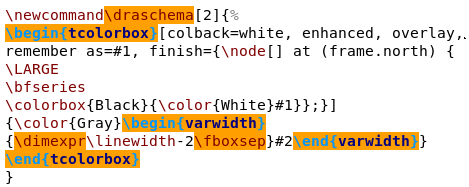
\includegraphics[scale=0.7]{Figures/Design/zmathb.png}
\caption{The syntax to define a \gls{zdra} schema instance in the \gls{zmath} \LaTeX{} file. \label{fig:latexzdraschema}}
\end{figure}

The new command we are defining for \verb|\draschema| is shown in figure
\ref{fig:latexzdraschema}. The commands for defining \verb|\dratheory| and
\verb|\draline| are similar as the \verb|draschema| definition. The command
takes two arguments, the first argument will be the name of the instance (e.g
SS1, IS4, CS2 etc) and the second argument is the instance itself. Any text
within the instance will then become grey so it looks faded as we are only
interested in the instance itself and not the context at this point. The
background of the box is white with a black outline. We then use the first
argument to name the instance and it becomes a node. The name of the instance is
also printed in black over the instance itself.

\subsection{\LaTeX{} commands to identify ZDRa Relations}

There are 5 new commands to define the relations for the \gls{zdra}, these are
\emph{initialOf}, \emph{uses}, \emph{totalises}, \emph{requires} and
\emph{requires}. Information on these relations are described in chapter
\ref{ch:zdra}, however this section of the thesis describes how the annotations
have been implemented in the \gls{zmath} \LaTeX{} package.

\begin{figure}[H]
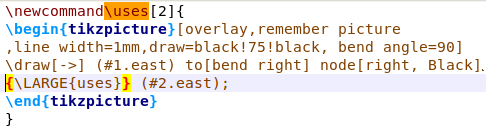
\includegraphics[scale=0.7]{Figures/Design/zmathd.png}
\caption{The syntax to define a \gls{zdra} schema relation in the \gls{zmath} \LaTeX{} file. \label{fig:latexzdrauses}}
\end{figure}

Figure \ref{fig:latexzdrauses} shows how the command \verb|uses| has been
implemented. The command takes 2 arguments (the should be 2 instances which have
been previously annotated) and draws an arrow going from the first instance to
the second one. The arrow bend angle is at 90, the arrow width is at 1mm and the
arrow goes from the east part of the first instance to the east part of the
second instance. The word \textbf{uses} is written next to the arrow. All the
other relation commands are written in a similar way however the direction of
the arrows differ and some arrows bend to the left whilst others bend to the
right. The bending of the arrows has been implemented at random so that the
compiled document has arrows showing on both sides of the theory and are not
overlapping too much.

\subsection{\LaTeX{} commands to identify ZCGa grammatical types}

The \gls{zcga} part of the \LaTeX{} file package uses the colours previously
defined in the style file. To define each of the grammatical types we use the
\texttt{fcolorbox} command. This creates a black outline and a coloured
background for each of the grammatical categories.

\begin{figure}[H]
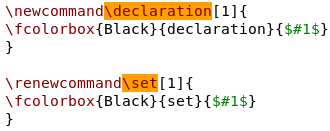
\includegraphics[scale=0.7]{Figures/Design/zmathe.png}
\caption{The syntax to define a \gls{zcga} grammatical categories. \label{fig:latexzcga}}
\end{figure}

Figure \ref{fig:latexzcga} shows the commands to define the coloured boxes for
\emph{declaration} and \emph{set}. As set is already defined in the mathematical
\LaTeX{} library, we renew the command. The command takes one argument (the text
the user which to annotate), changes it to mathmode and draws the box around it.
All the grammatical categories are defined in the same way, each with their own
background colour. The only exception is the grammatical category of
\emph{specification} as this command does not convert the specification into
mathmode.

\section{Conclusion}

In total there are 6 steps in order to translate a Z specification into the
theorem prover Isabelle. These steps have been designed so that the system
engineer/system designer of the project could use them.  Each of these steps
assist the user in understanding the specification, and some steps even produce
documents, graphs and charts in order to analyse the specification. These
products also allow others in the development team to understand the system
better such as clients, stakeholders, developers etc. The majority of the steps
are fully automated whilst some a little user input. Each step checks for some
form of correctness and becomes more and more rigorous each step the user takes
towards step 6. The next chapter begins to describe step 1 (\gls{zcga}) in more
detail.